% filepath: c:\Users\isiva\Documents\donammon\tex\resultados.tex

Para ofrecer una visión clara del funcionamiento, se explica a continuación cómo el usuario interactúa con la aplicación desde que la abre hasta que finaliza su uso.

El punto de partida es la pantalla de bienvenida, tal como se observa en la Figura~\ref{fig:captura1}. También vemos cómo ha saltado la notificación de que nos encontramos cerca de un lugar.

\begin{figure}[H]
    \centering
    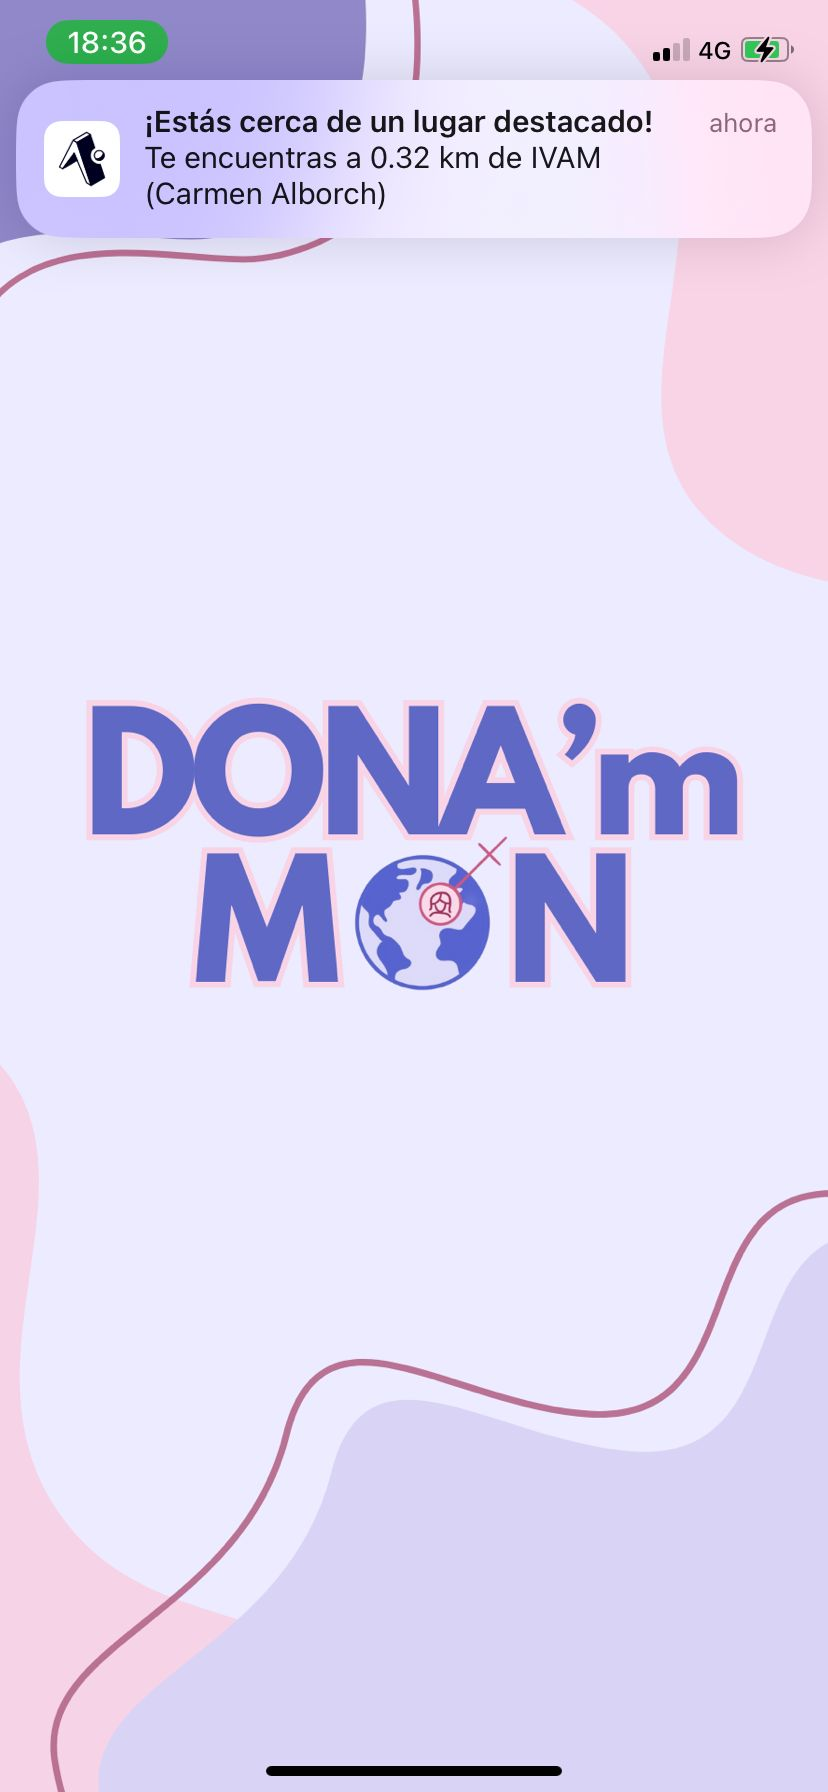
\includegraphics[width=0.3\textwidth]{figs/captura1.jpg}
    \caption{Pantalla de bienvenida y notificación de proximidad a un lugar.}
    \label{fig:captura1}
\end{figure}

En la Figura~\ref{fig:captura2} se ve el mapa con los lugares visitados en verde y los no visitados en rosa, además de nuestra ubicación.

\begin{figure}[H]
    \centering
    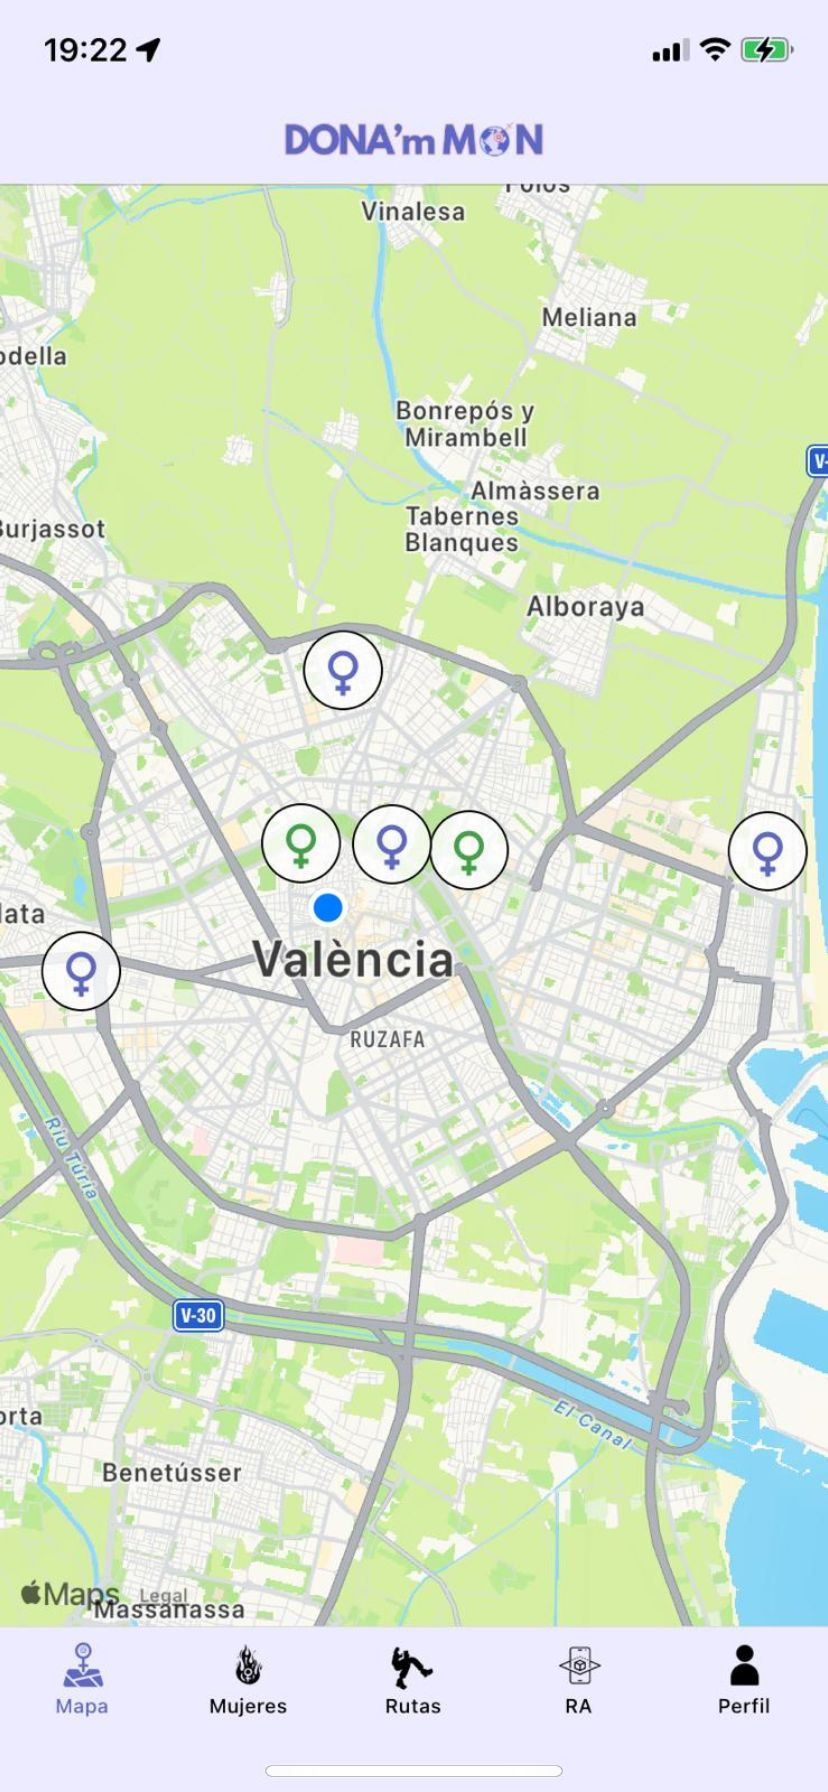
\includegraphics[width=0.3\textwidth]{figs/captura2.jpg}
    \caption{Mapa con lugares visitados (verde), no visitados (rosa) y ubicación actual.}
    \label{fig:captura2}
\end{figure}

Al pulsar sobre un lugar se muestra la información de la mujer y el lugar, además de la distancia (Figura~\ref{fig:captura3}).

\begin{figure}[H]
    \centering
    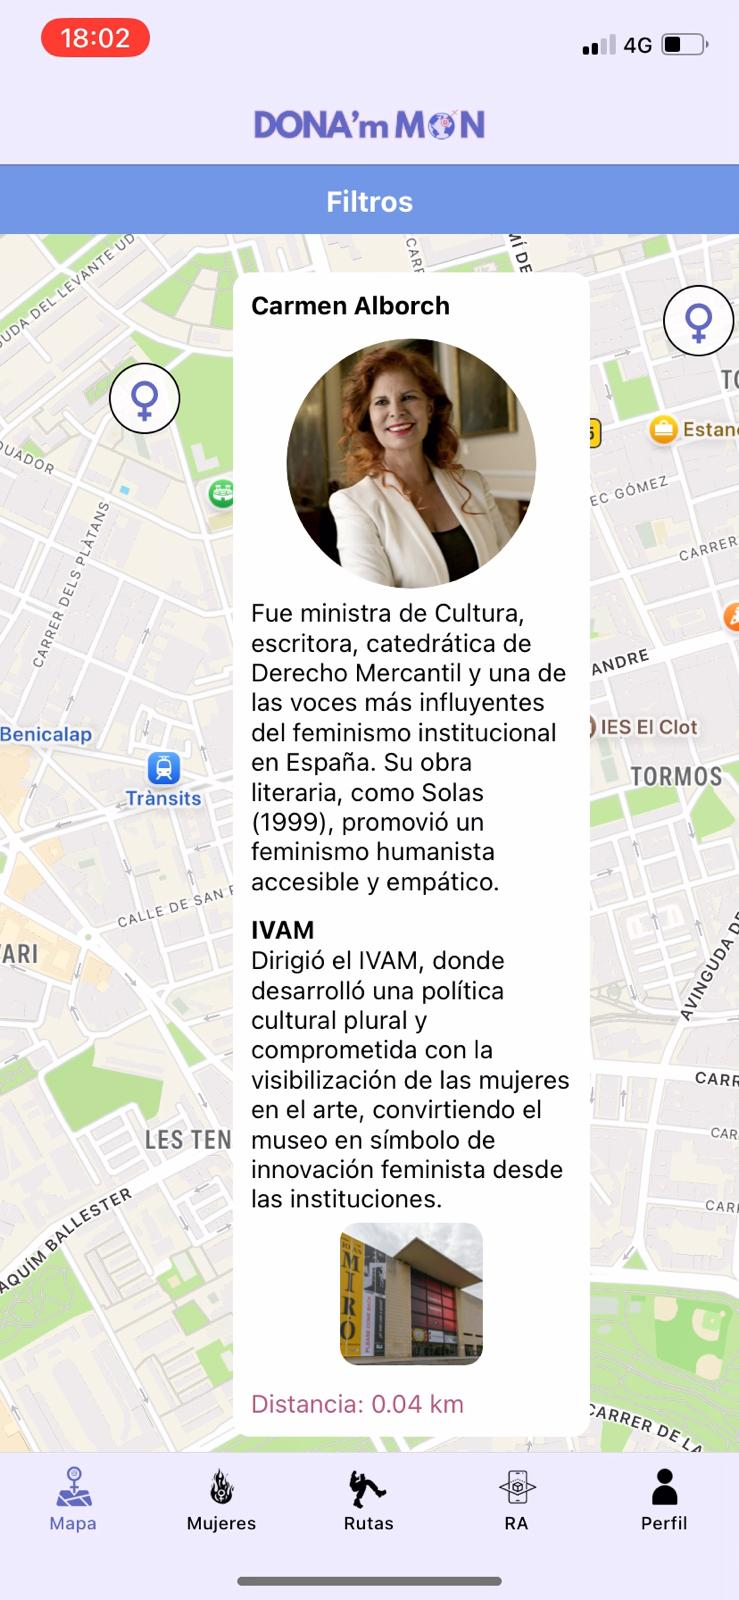
\includegraphics[width=0.3\textwidth]{figs/captura3.jpg}
    \caption{Detalle de un lugar: información de la mujer, el lugar y distancia.}
    \label{fig:captura3}
\end{figure}

En la Figura~\ref{fig:captura4} se ve el listado de lugares, y también podemos observar el buscador por nombre de lugares y de mujeres.

\begin{figure}[H]
    \centering
    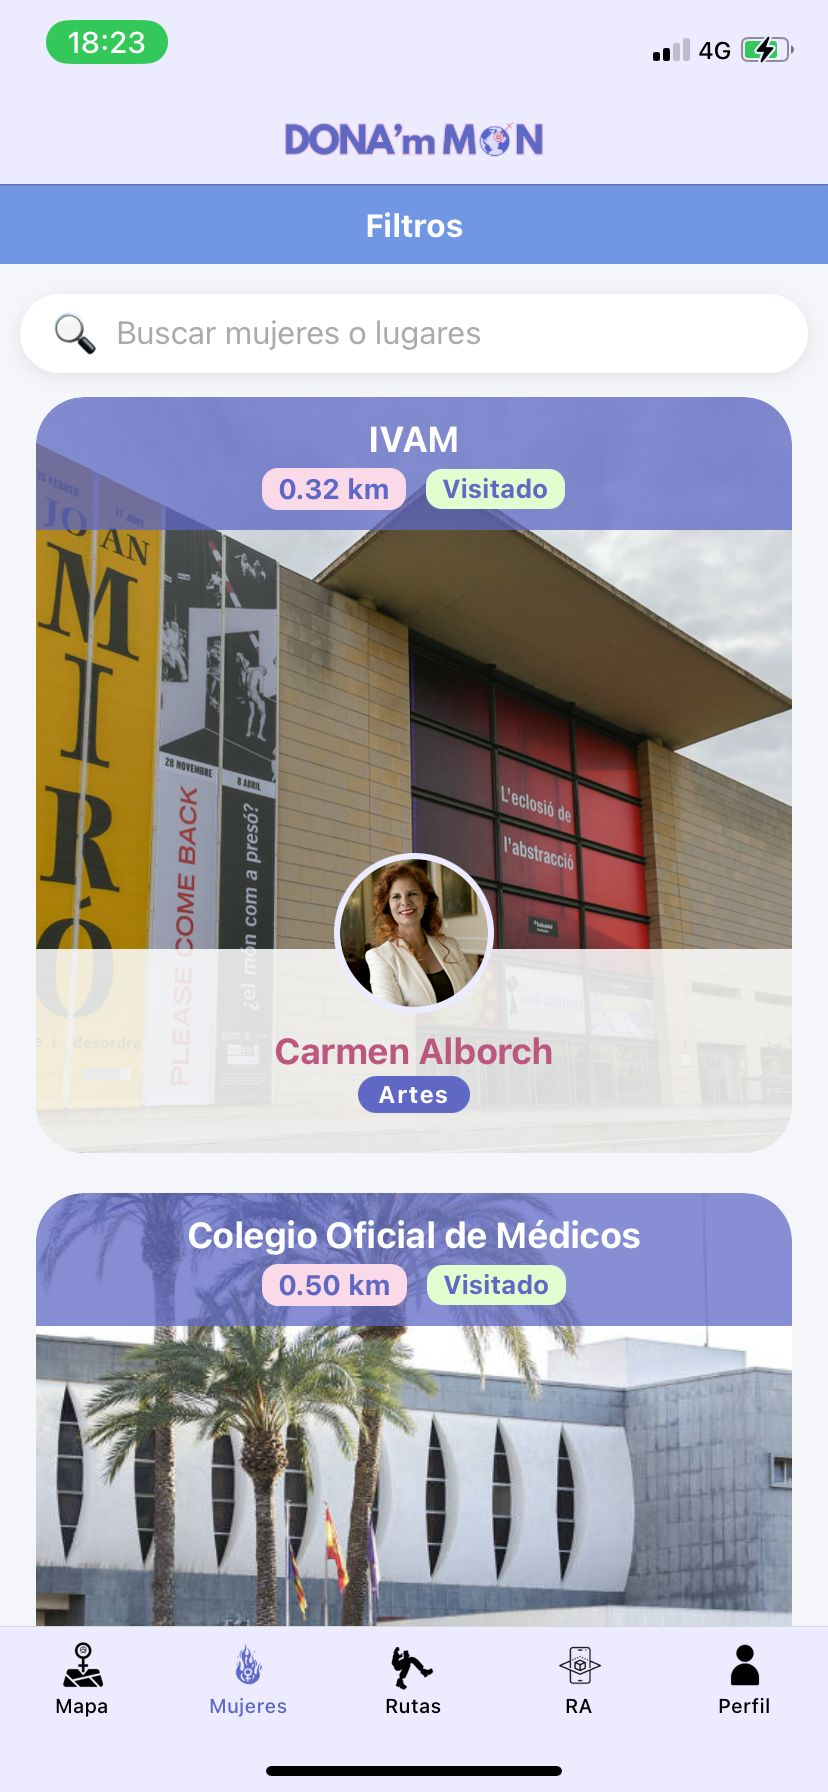
\includegraphics[width=0.3\textwidth]{figs/captura4.jpg}
    \caption{Listado de lugares y buscador por nombre de lugares y mujeres.}
    \label{fig:captura4}
\end{figure}

En la Figura~\ref{fig:captura_filtros} observamos los filtros que podemos aplicar tanto sobre el mapa como sobre el listado de lugares.

\begin{figure}[H]
    \centering
    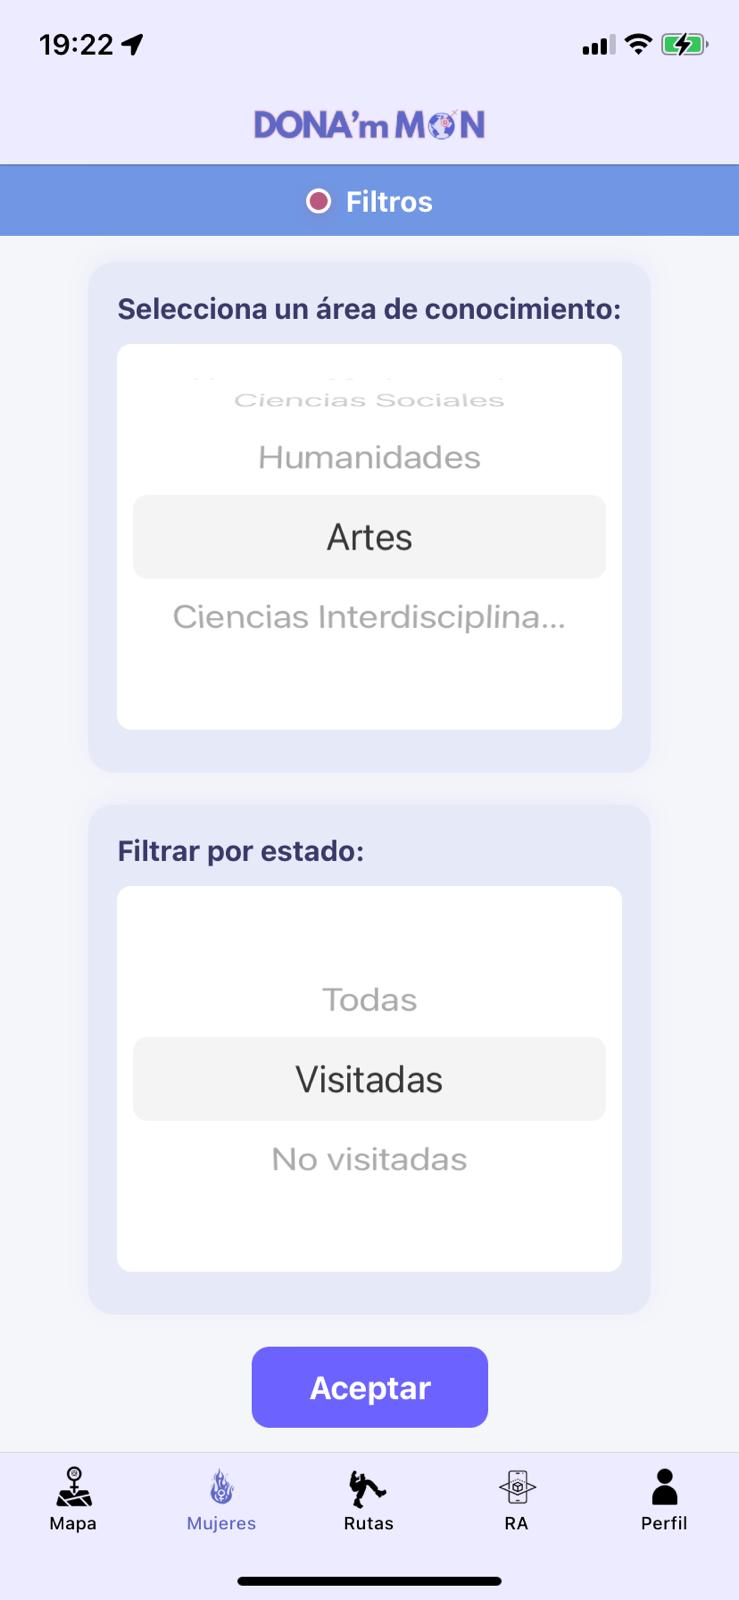
\includegraphics[width=0.3\textwidth]{figs/captura_filtros.jpg}
    \caption{Filtros aplicables sobre el mapa y el listado de lugares.}
    \label{fig:captura_filtros}
\end{figure}

En las Figuras~\ref{fig:captura5} y~\ref{fig:captura6} se muestra el detalle de un lugar, pudiendo marcar como visitado libremente o compartir el lugar, como se ve en las Figuras~\ref{fig:captura7} y~\ref{fig:capturawats}.
\begin{figure}[H]
    \centering
    \begin{subfigure}[b]{0.45\textwidth}
        \centering
        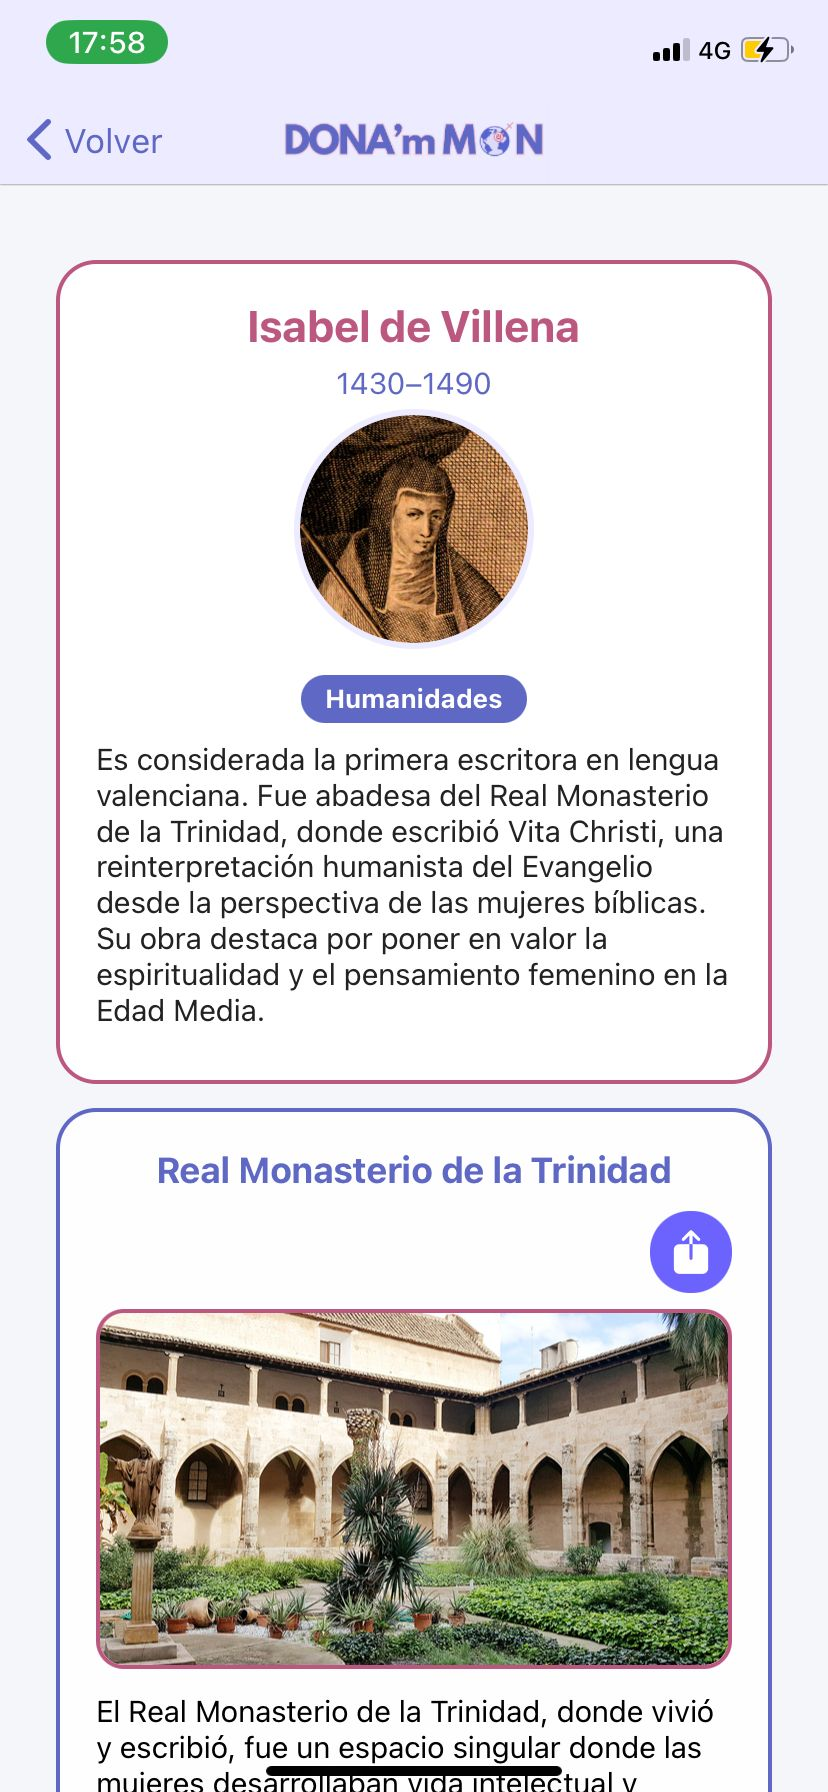
\includegraphics[width=0.65\linewidth]{figs/captura5.jpg}
        \caption{Detalle de un lugar (1).}
        \label{fig:captura5}
    \end{subfigure}
    \hfill
    \begin{subfigure}[b]{0.45\textwidth}
        \centering
        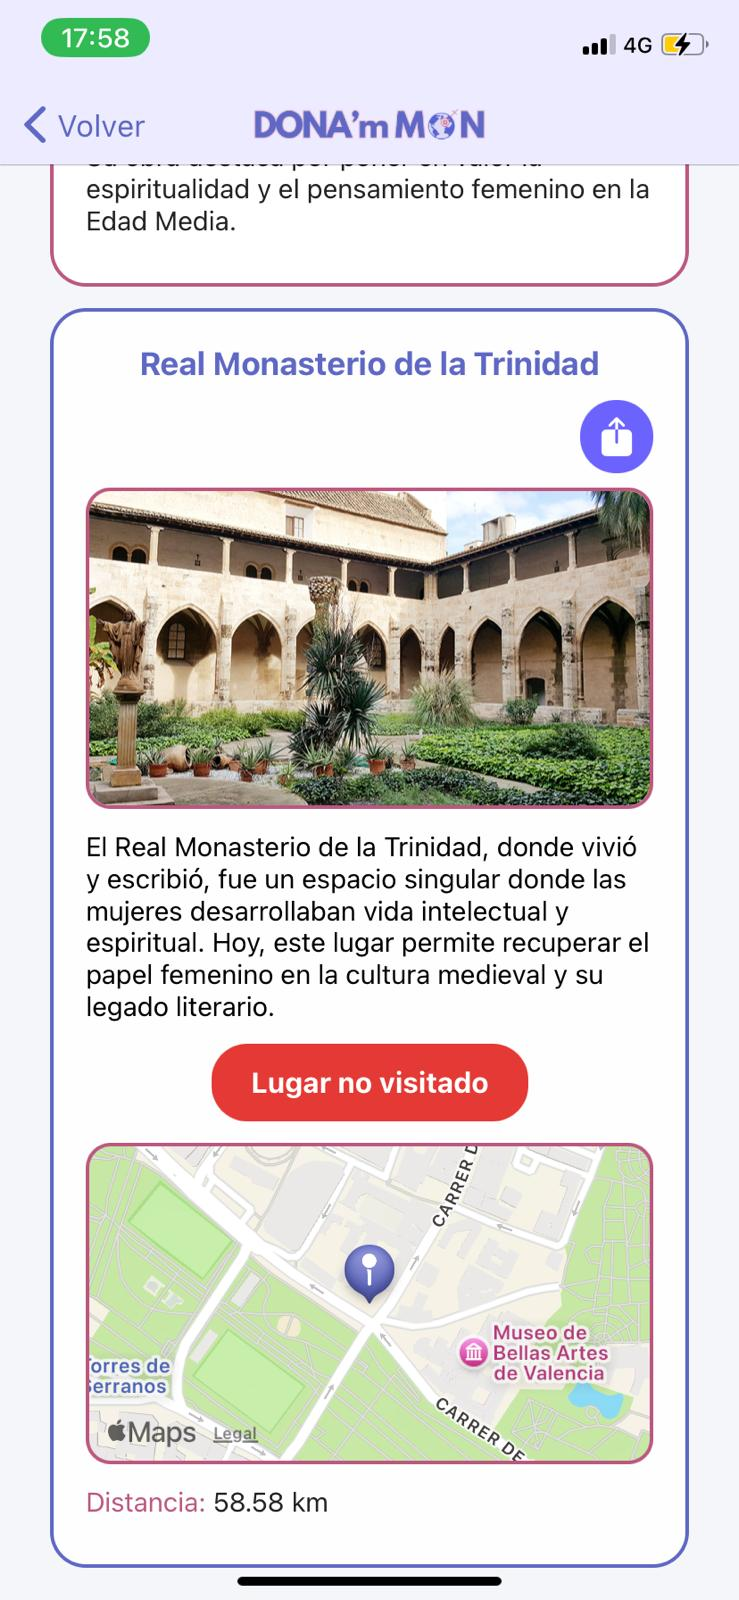
\includegraphics[width=0.65\linewidth]{figs/captura6.jpg}
        \caption{Detalle de un lugar (2).}
        \label{fig:captura6}
    \end{subfigure}
    \caption{Detalles de un lugar en la aplicación.}
\end{figure}

\begin{figure}[H]
    \centering
    \begin{subfigure}[b]{0.45\textwidth}
        \centering
        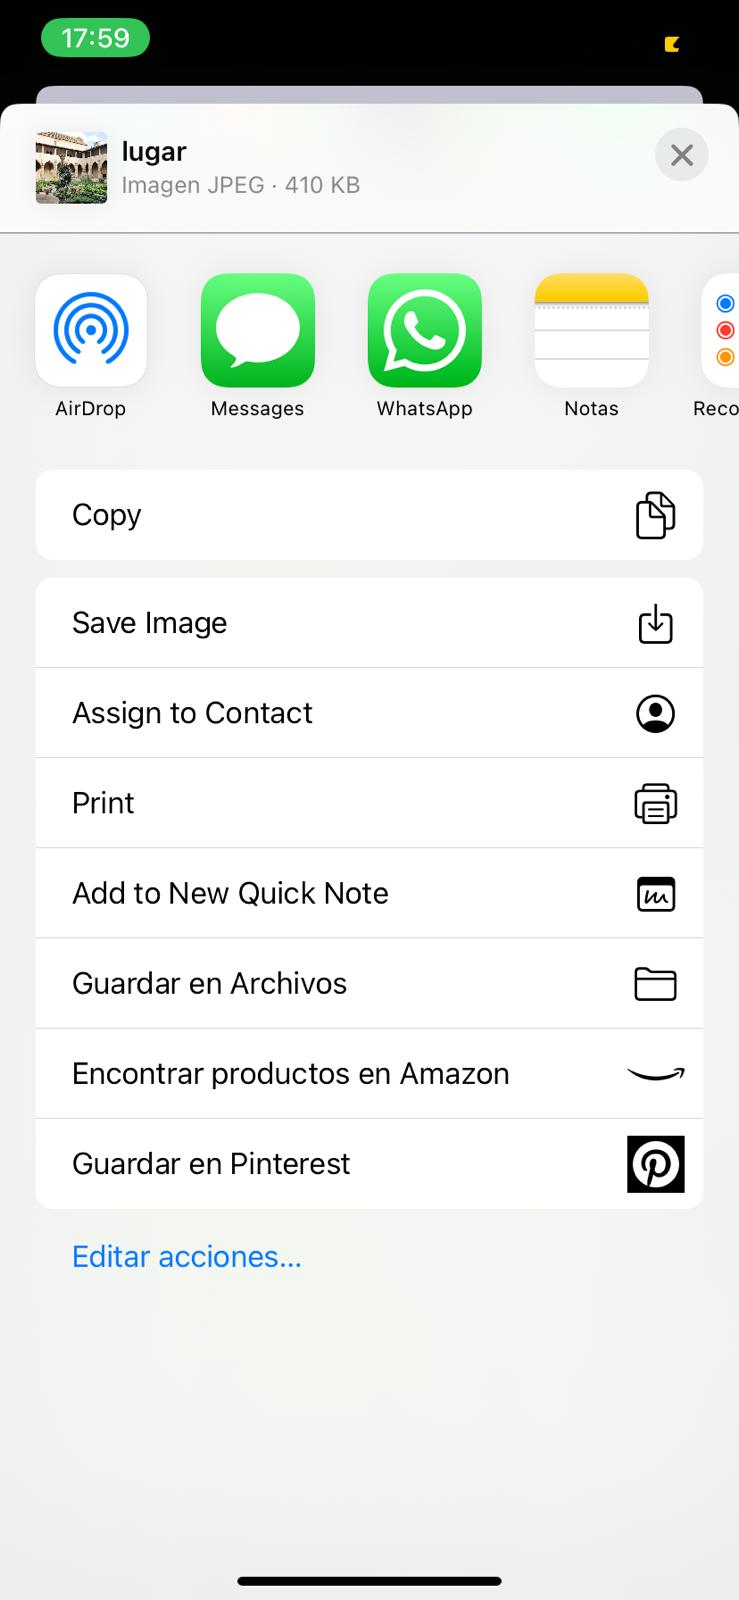
\includegraphics[width=0.65\linewidth]{figs/captura7.jpg}
        \caption{Opción para compartir el lugar (1).}
        \label{fig:captura7}
    \end{subfigure}
    \hfill
    \begin{subfigure}[b]{0.45\textwidth}
        \centering
        
\includegraphics[width=0.65\linewidth]{figs/capturawats.jpg}
        \caption{Opción para compartir el lugar (2).}
        \label{fig:capturawats}
    \end{subfigure}
    \caption{Opciones de interacción con el lugar: compartir.}
\end{figure}

En la Figura~\ref{fig:captura_modal} se observa cómo se muestran las imágenes al pulsar sobre ellas.

\begin{figure}[H]
    \centering
    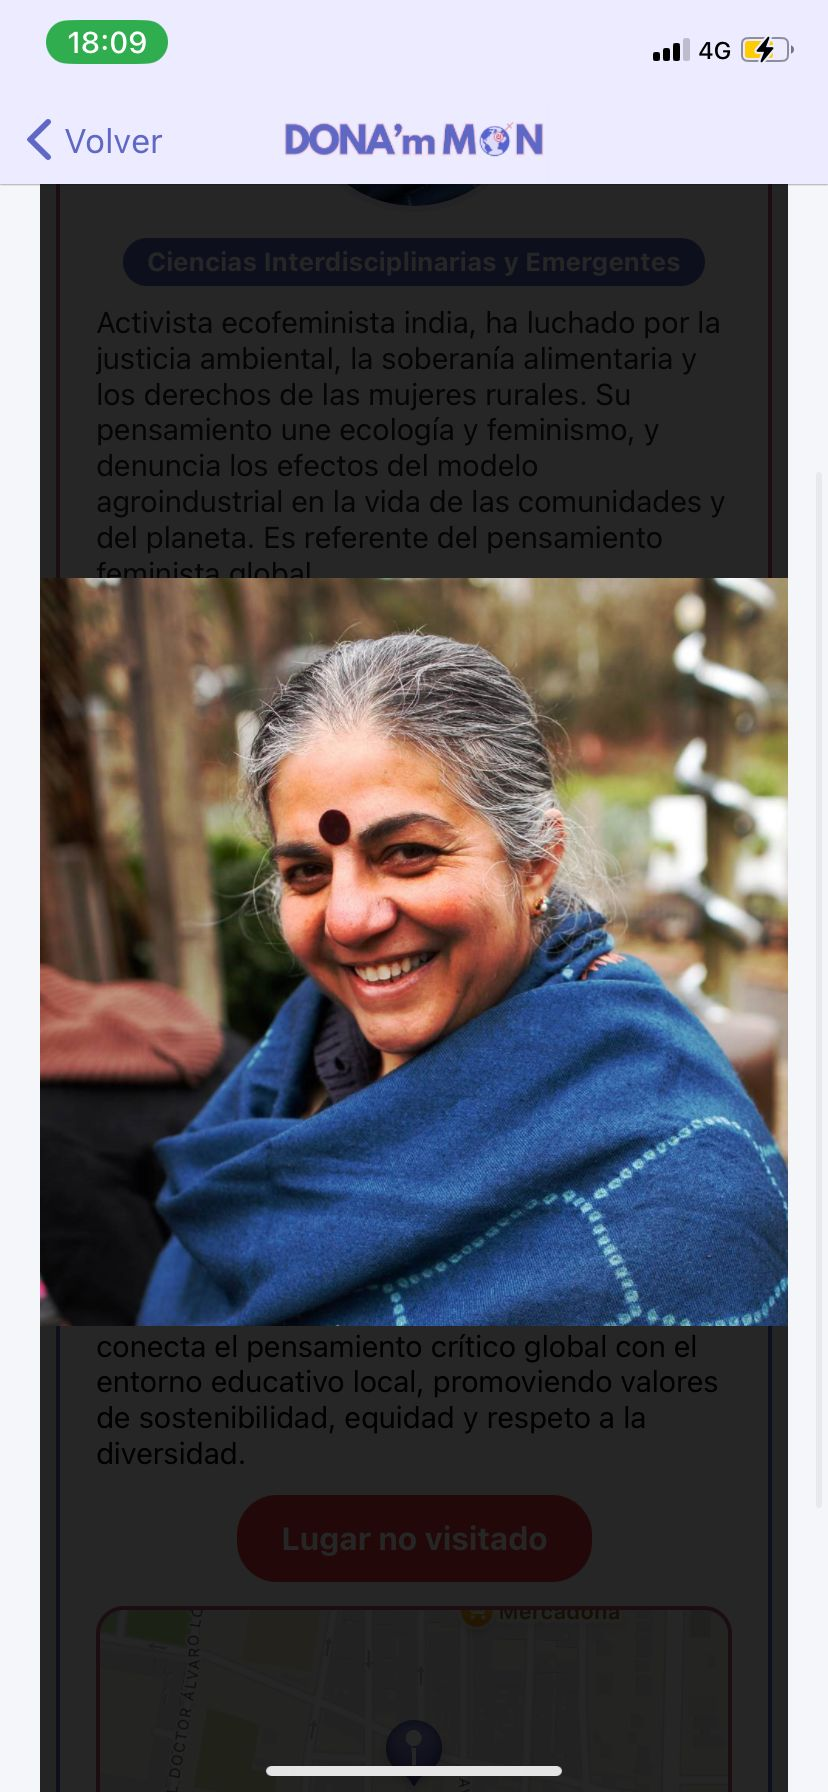
\includegraphics[width=0.3\textwidth]{figs/captura_modal.jpg}
    \caption{Visualización de imágenes en modal.}
    \label{fig:captura_modal}
\end{figure}

En la Figura~\ref{fig:captura8} se muestra la página de rutas, en la Figura~\ref{fig:captura9} una ruta incompleta y en la Figura~\ref{fig:captura10} una ruta completada escaneando un código QR que se obtiene al llegar al lugar.

\begin{figure}[H]
    \centering
    \begin{subfigure}[b]{0.3\textwidth}
        \centering
        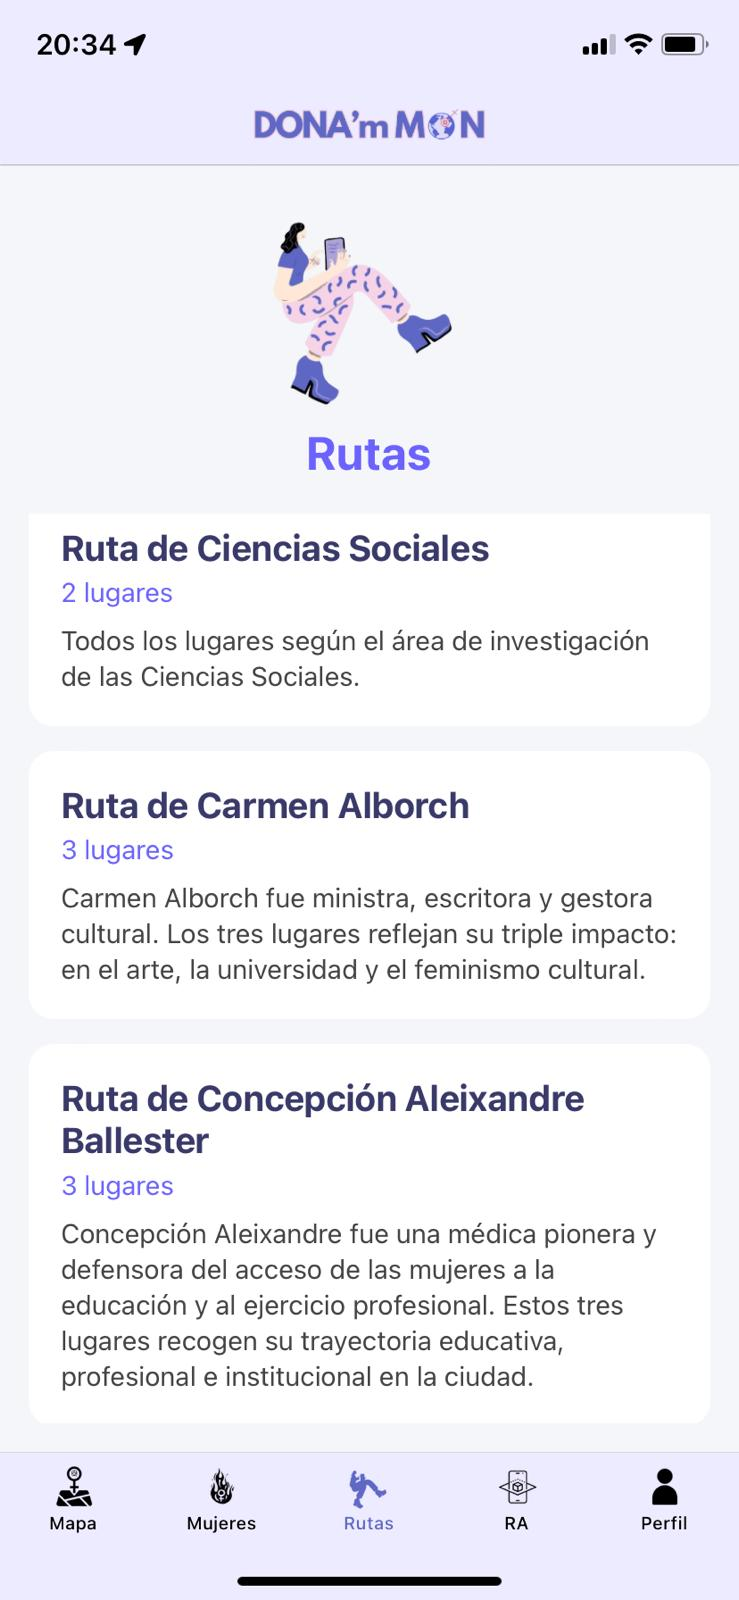
\includegraphics[width=0.9\linewidth]{figs/captura8.jpg}
        \caption{Página de rutas.}
        \label{fig:captura8}
    \end{subfigure}
    \hfill
    \begin{subfigure}[b]{0.3\textwidth}
        \centering
        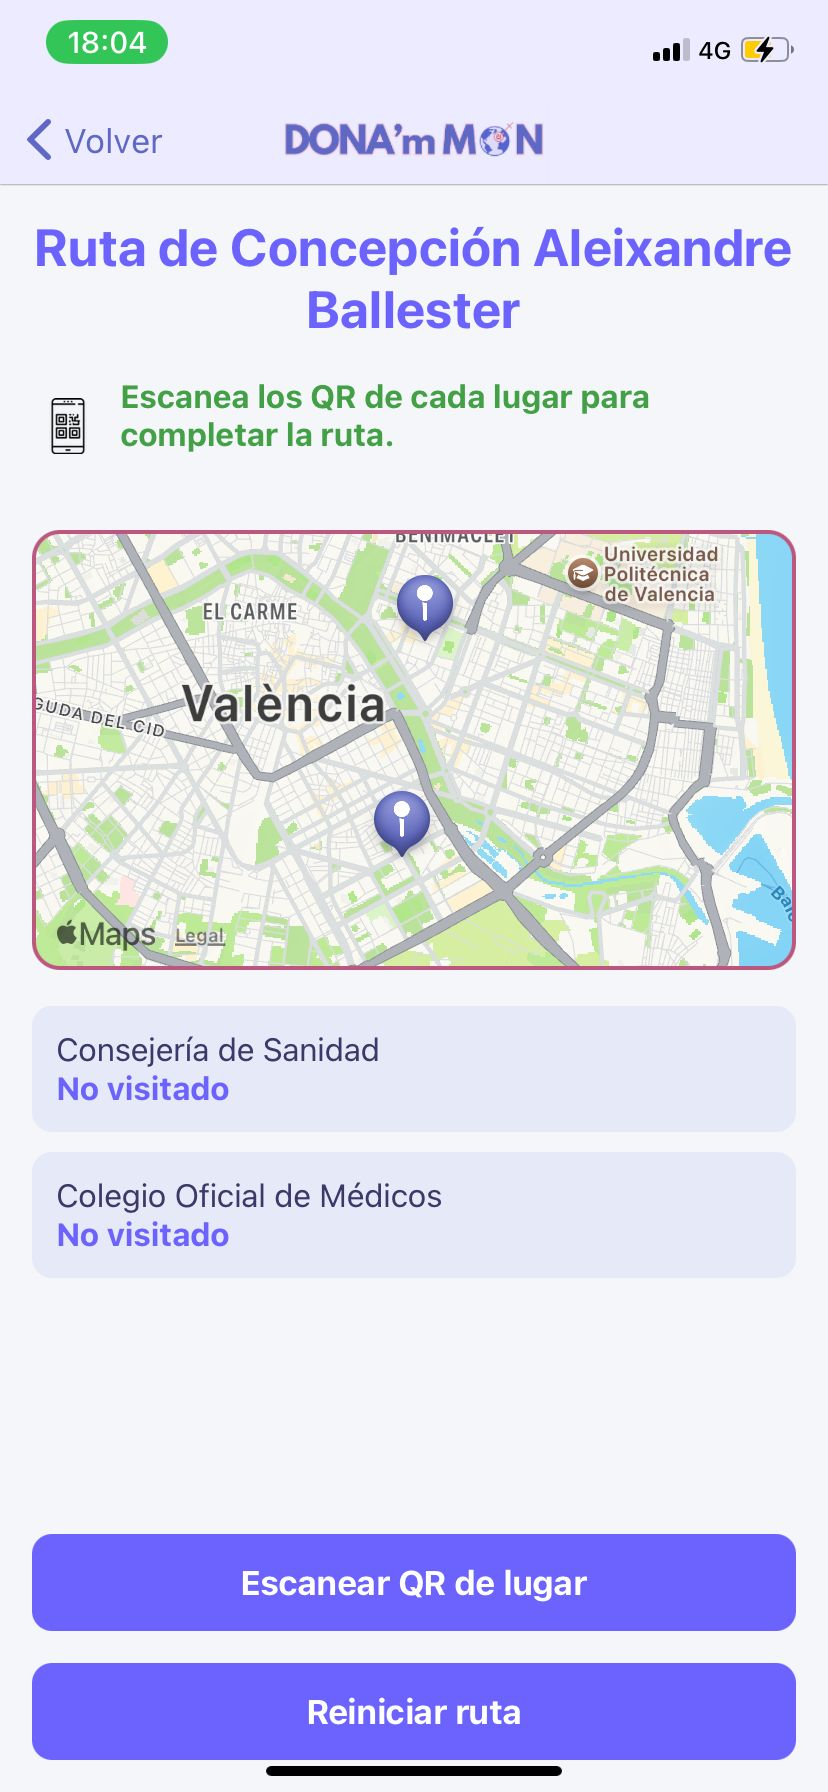
\includegraphics[width=0.9\linewidth]{figs/captura9.jpg}
        \caption{Ruta incompleta.}
        \label{fig:captura9}
    \end{subfigure}
    \hfill
    \begin{subfigure}[b]{0.3\textwidth}
        \centering
        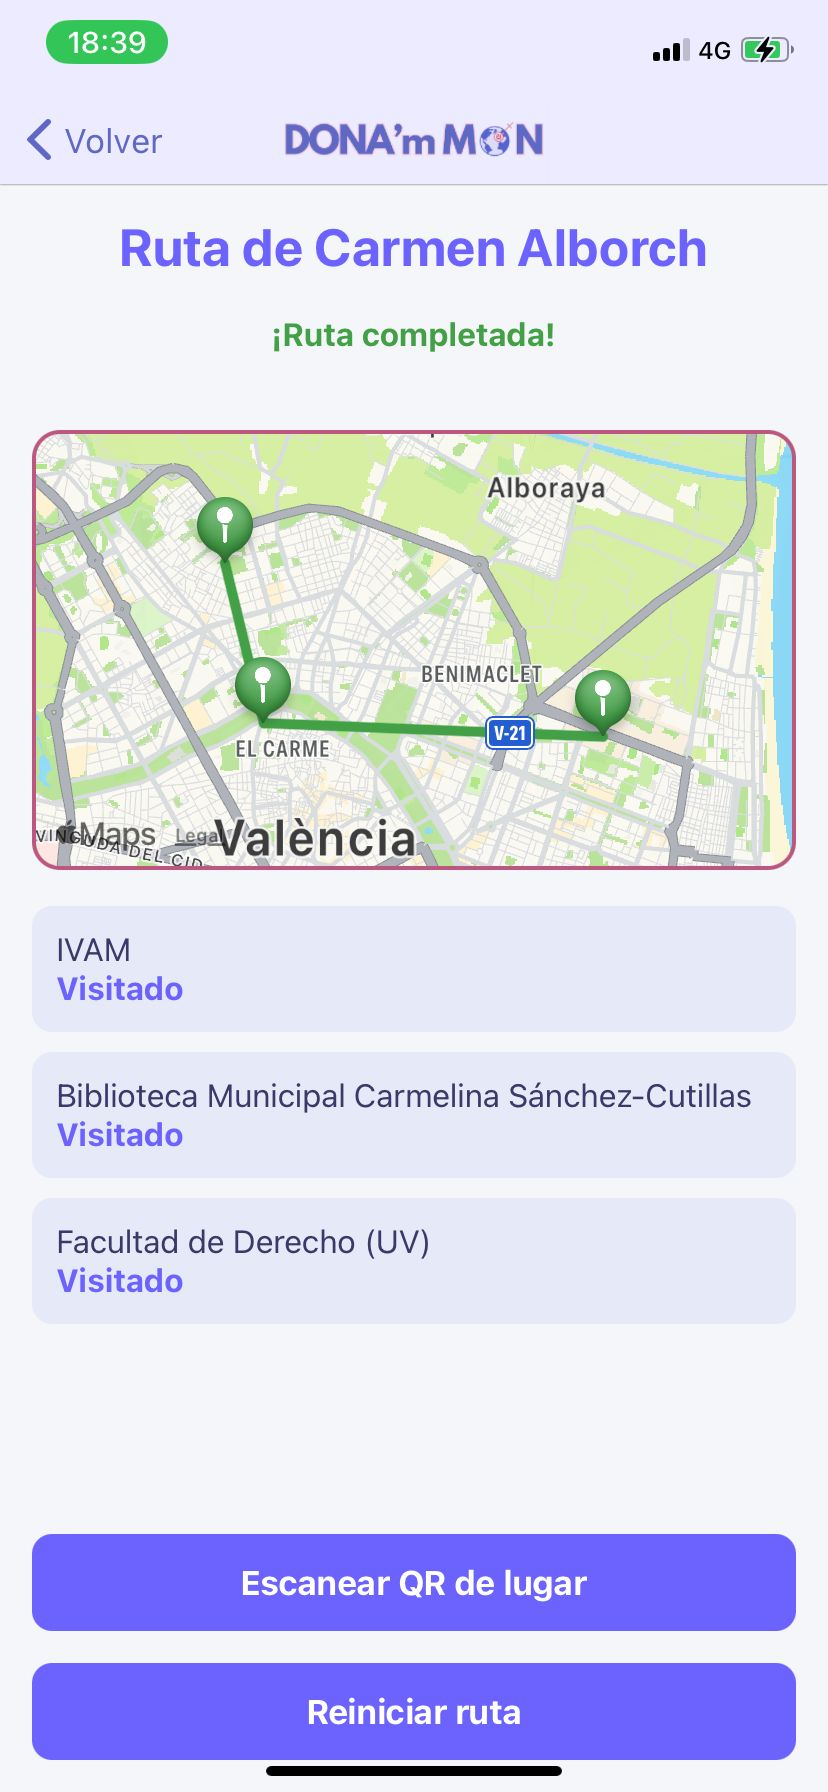
\includegraphics[width=0.9\linewidth]{figs/captura10.jpg}
        \caption{Ruta completada.}
        \label{fig:captura10}
    \end{subfigure}
    \caption{Página de rutas y ejemplos de rutas incompleta y completada.}
\end{figure}


La Figura~\ref{fig:captura11} muestra la pantalla de realidad aumentada, y las Figuras~\ref{fig:captura12},~\ref{fig:captura13} y~\ref{fig:captura14} la experiencia de realidad aumentada.

\begin{figure}[H]
    \centering
    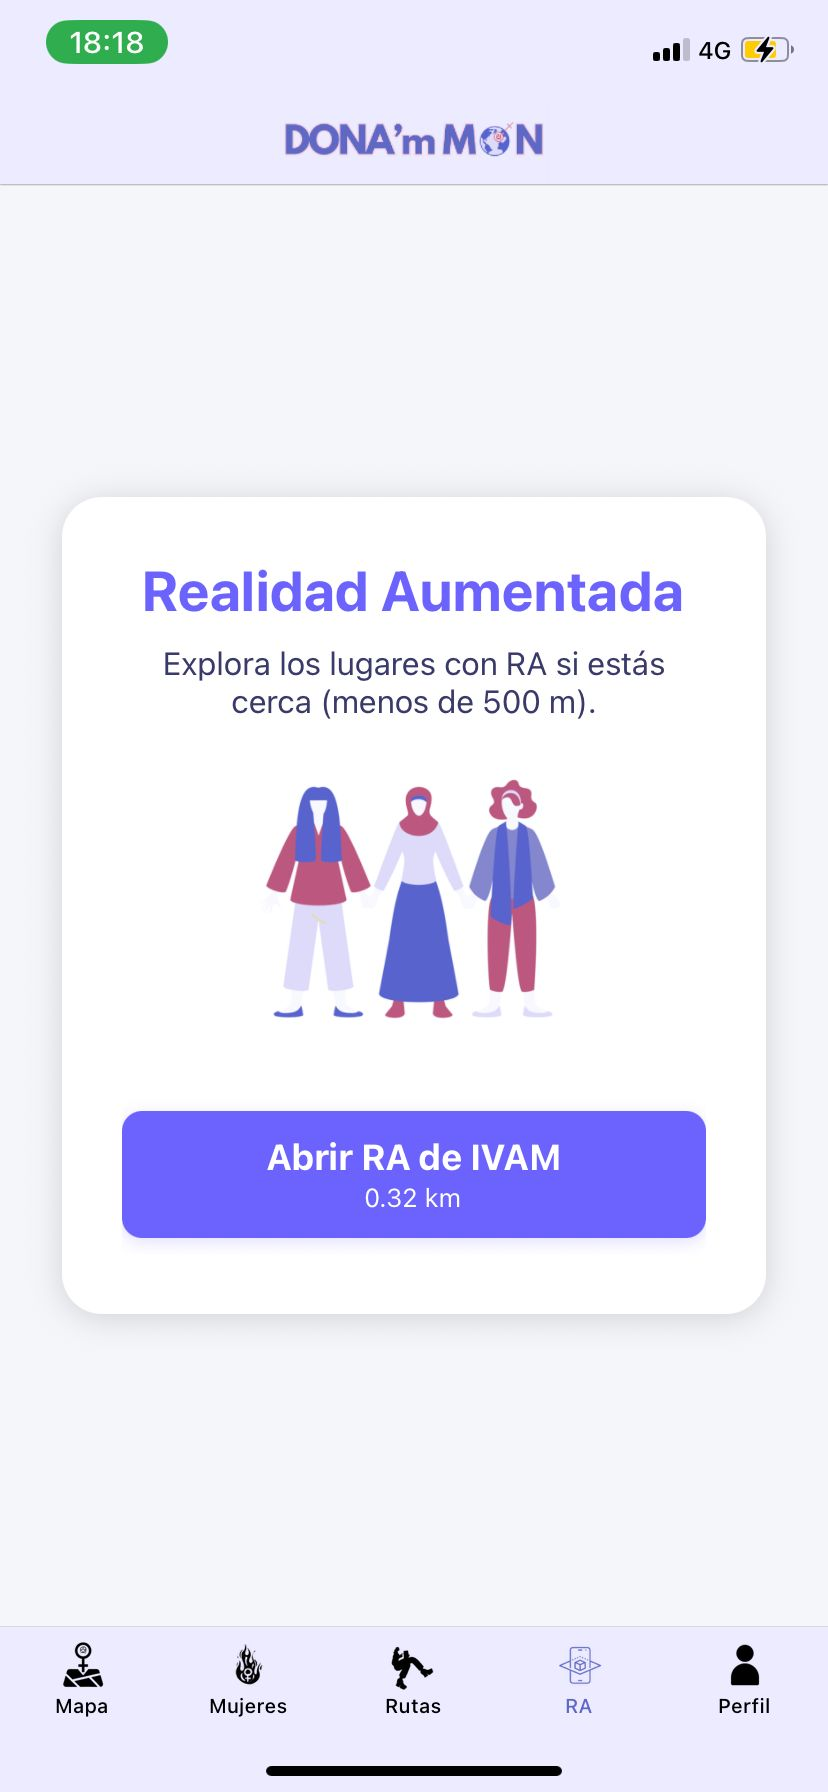
\includegraphics[width=0.3\textwidth]{figs/captura11.jpg}
    \caption{Pantalla de realidad aumentada.}
    \label{fig:captura11}
\end{figure}

\begin{figure}[H]
    \centering
    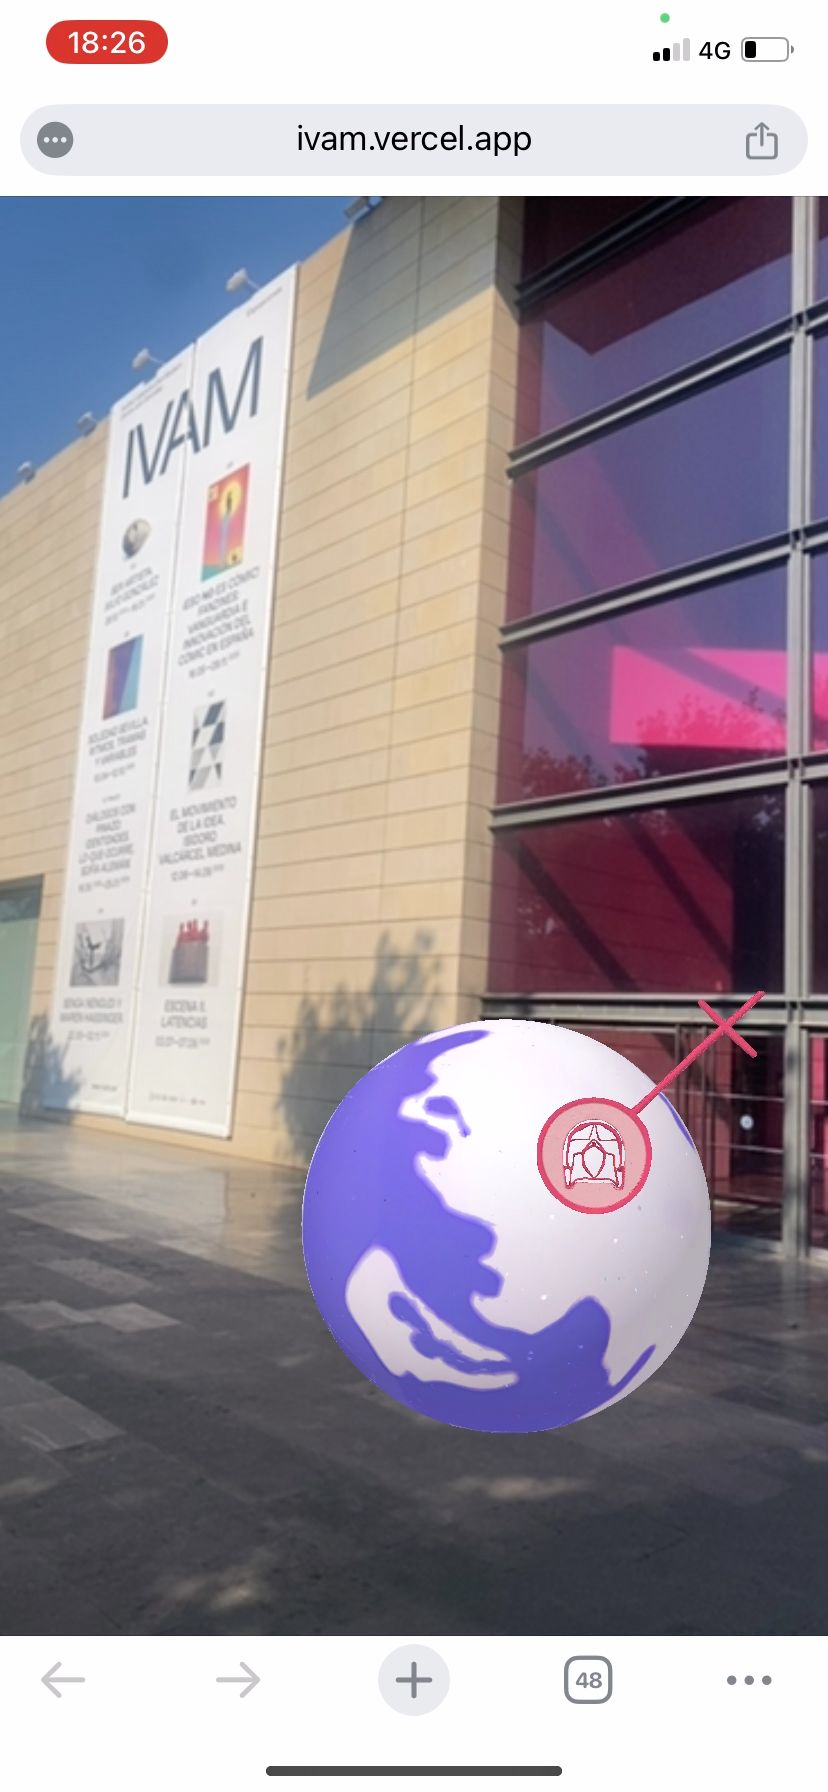
\includegraphics[width=0.3\textwidth]{figs/captura12.jpg}
    \caption{Experiencia de realidad aumentada (1).}
    \label{fig:captura12}
\end{figure}

\begin{figure}[H]
    \centering
    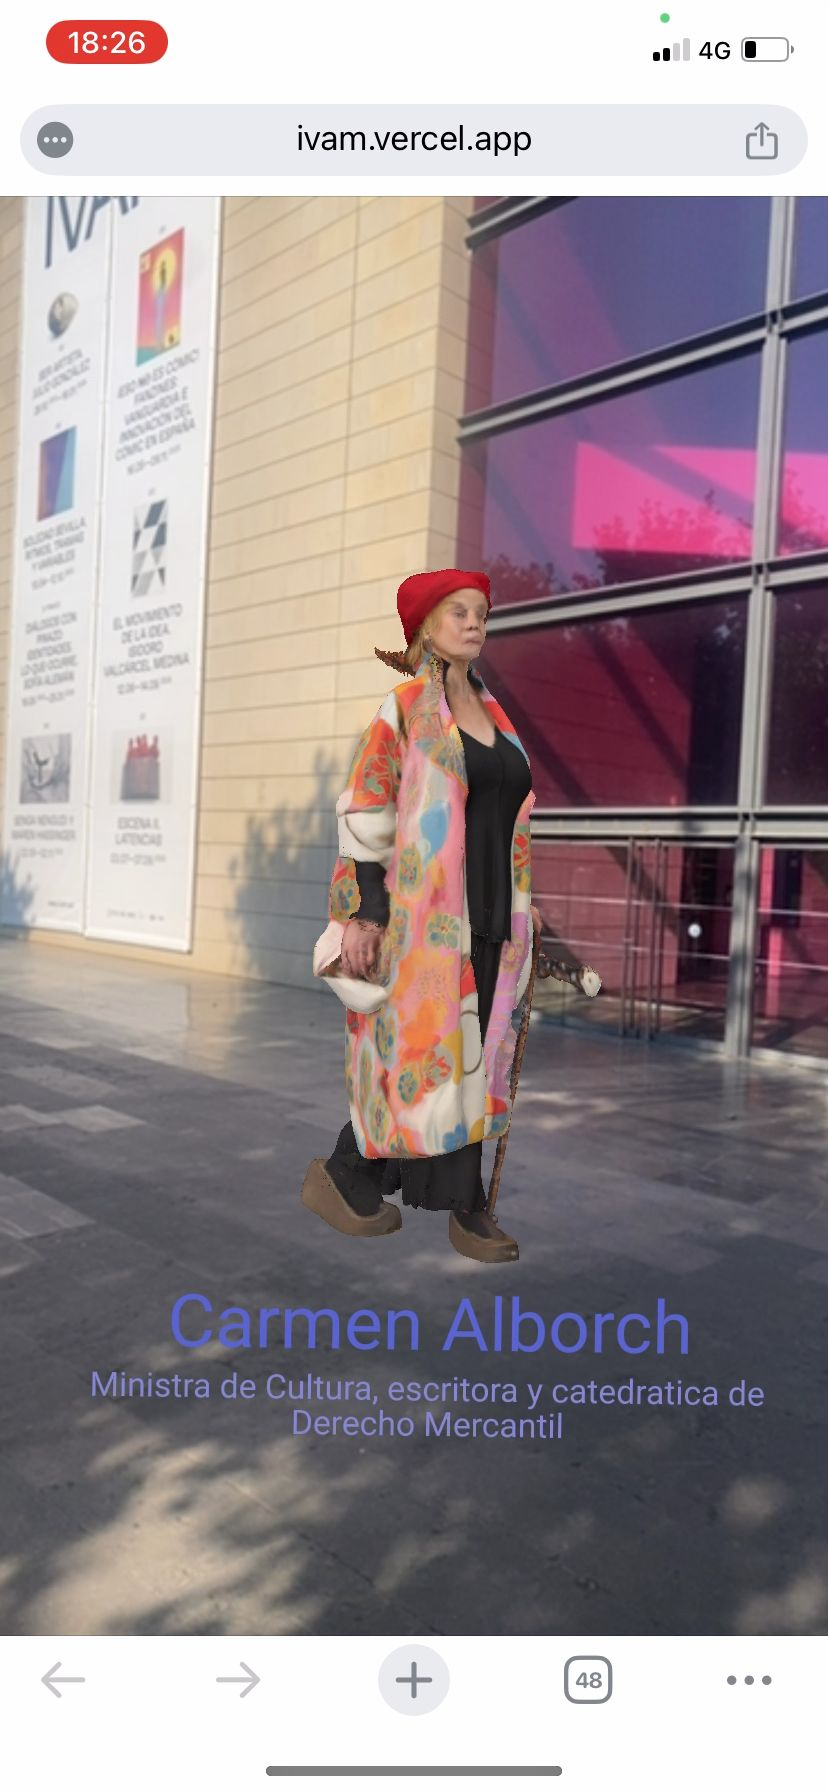
\includegraphics[width=0.3\textwidth]{figs/captura13.jpg}
    \caption{Experiencia de realidad aumentada (2).}
    \label{fig:captura13}
\end{figure}

\begin{figure}[H]
    \centering
    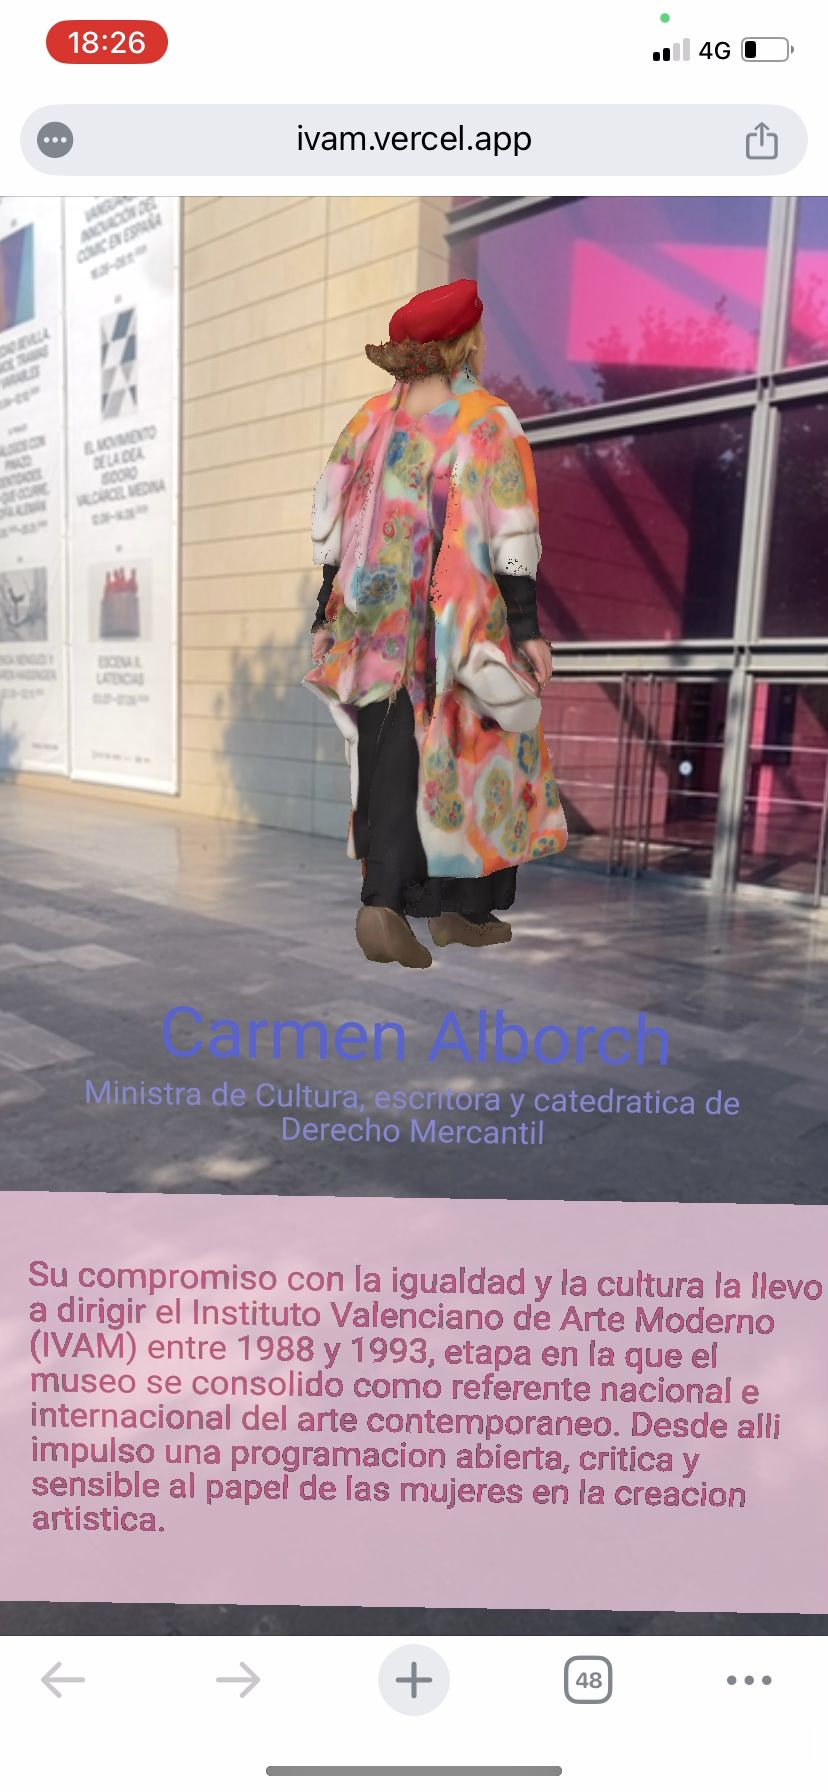
\includegraphics[width=0.3\textwidth]{figs/captura14.jpg}
    \caption{Experiencia de realidad aumentada (3).}
    \label{fig:captura14}
\end{figure}

Por último, la Figura~\ref{fig:captura15} muestra la pantalla de perfil, donde el usuario puede modificar su nombre, acceder al historial de sus lugares visitados (Figura~\ref{fig:captura16}), al historial de las rutas completas (Figura~\ref{fig:captura17}) y cerrar sesión. Si se pulsa en borrar en alguno de los historiales, se actualizará el mapa, el listado o las rutas también.

\begin{figure}[H]
    \centering
    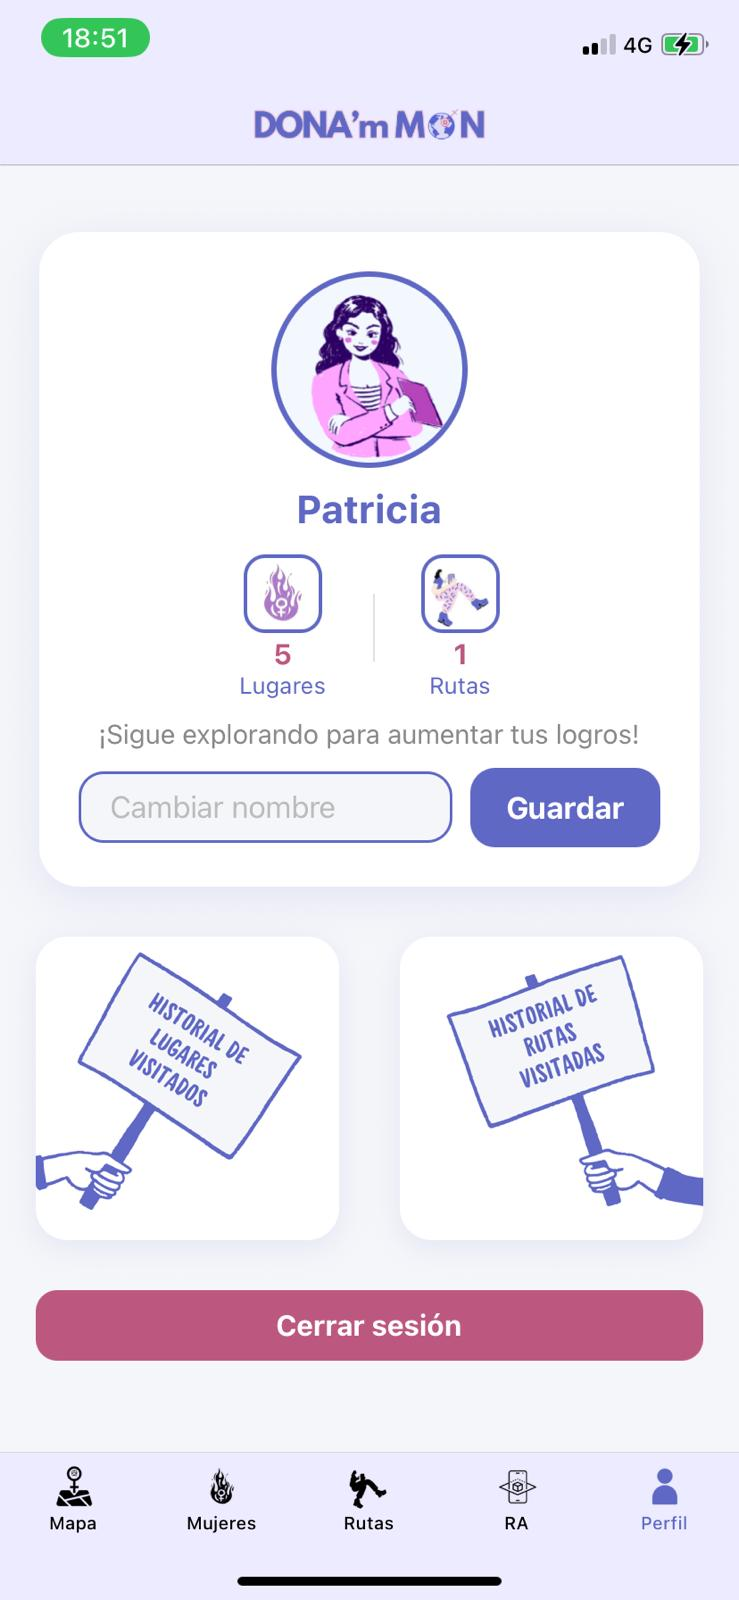
\includegraphics[width=0.3\textwidth]{figs/captura15.jpg}
    \caption{Pantalla de perfil del usuario.}
    \label{fig:captura15}
\end{figure}

\begin{figure}[H]
    \centering
    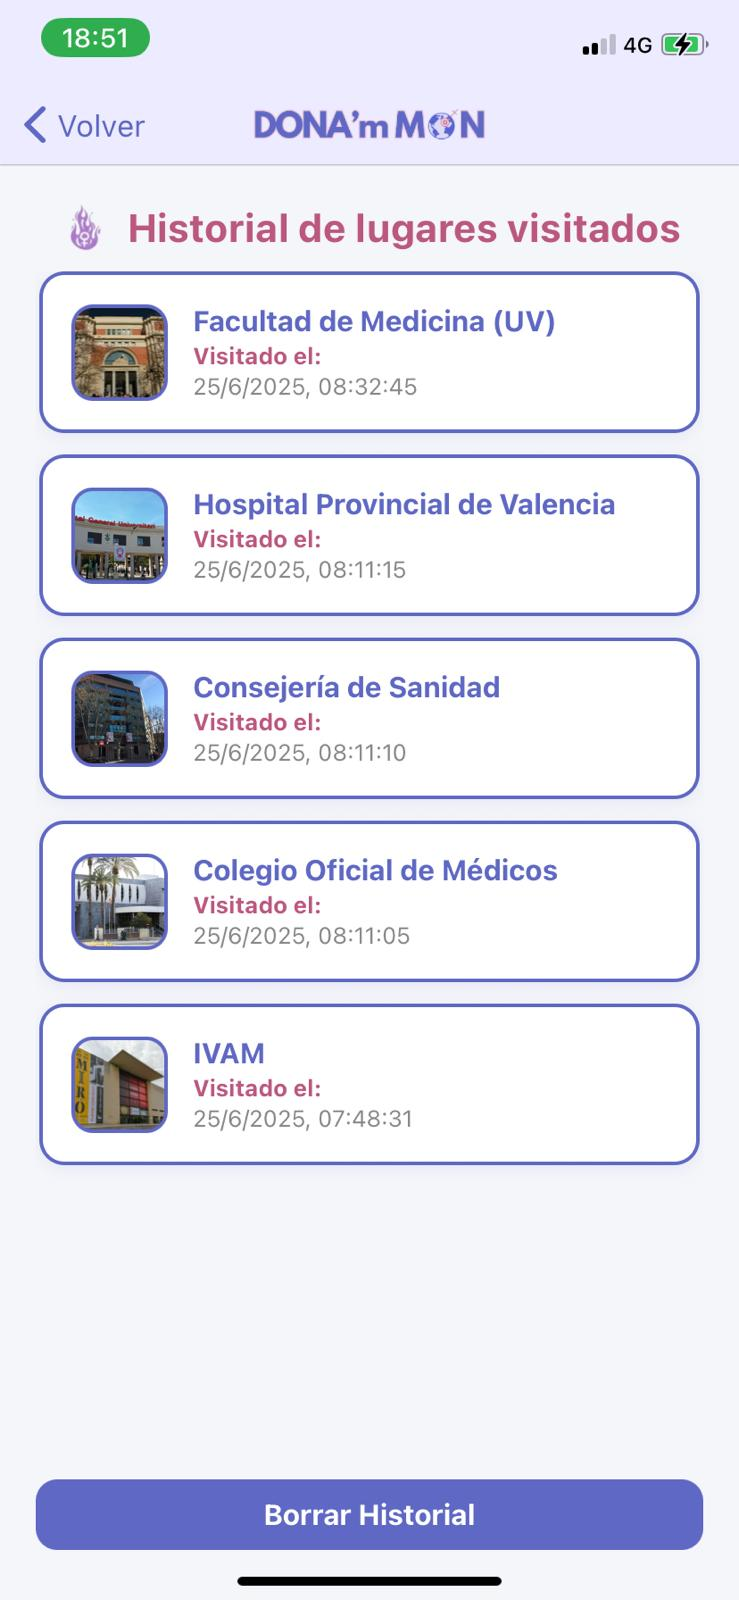
\includegraphics[width=0.3\textwidth]{figs/captura16.jpg}
    \caption{Historial de lugares visitados.}
    \label{fig:captura16}
\end{figure}

\begin{figure}[H]
    \centering
    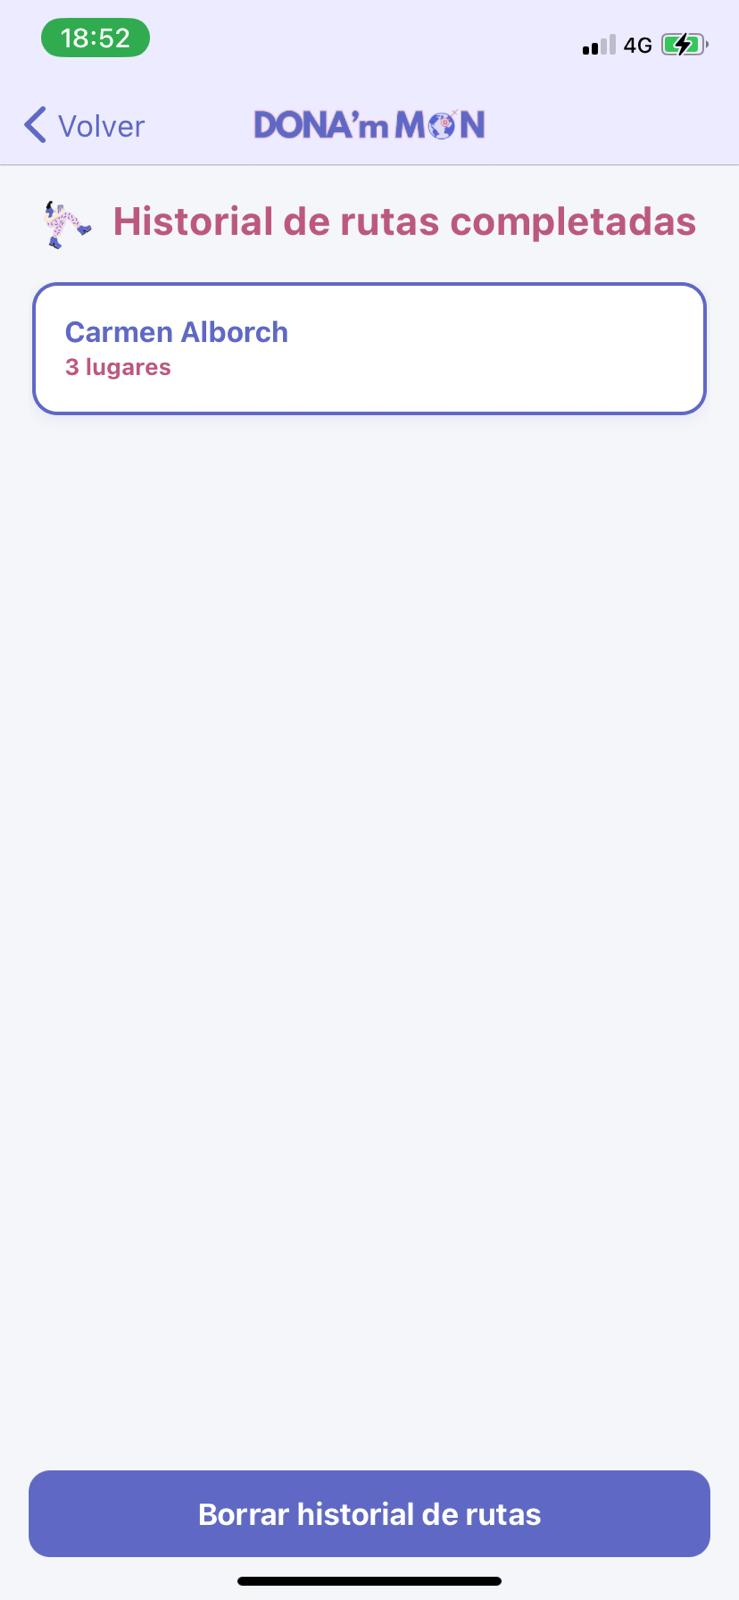
\includegraphics[width=0.3\textwidth]{figs/captura17.jpg}
    \caption{Historial de rutas completadas.}
    \label{fig:captura17}
\end{figure}
